\subsubsection{Use case diagram}
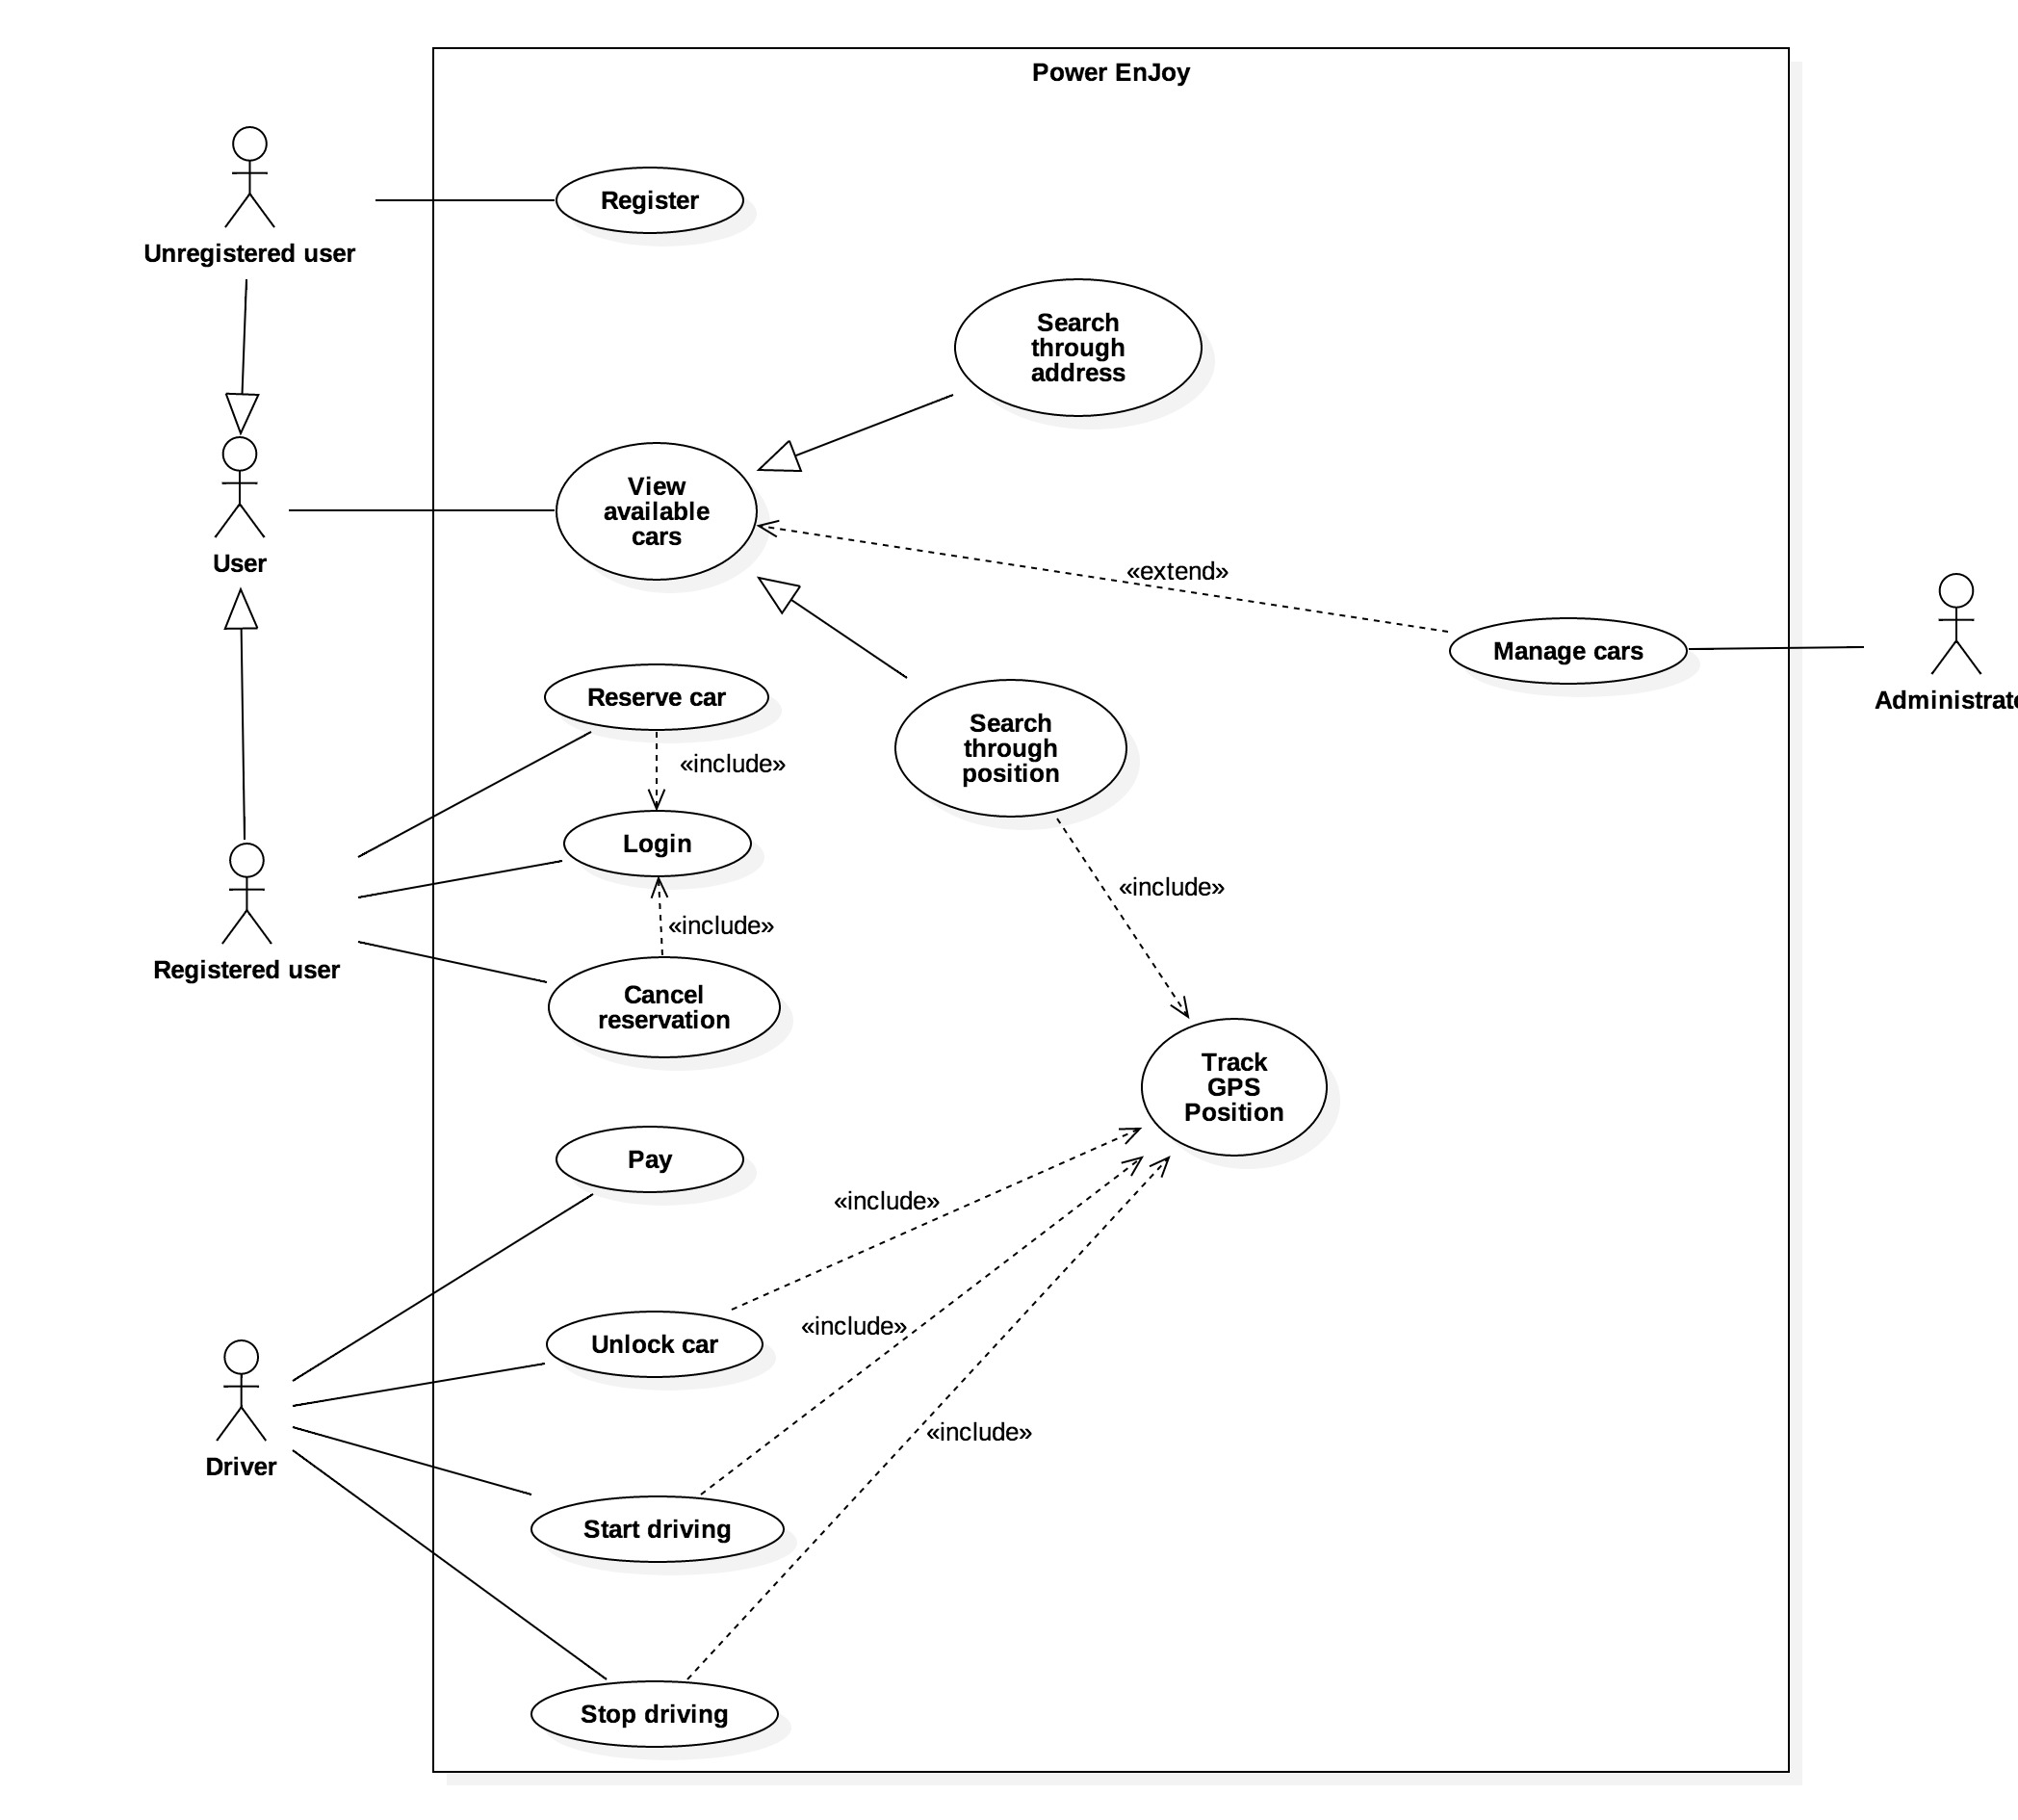
\includegraphics[width=\textwidth]{UseCaseDiagram2}


\subsubsection{Register account}

\begin{center}
	\begin{tabular}{c | p{.8\textwidth} }
		\hline
		\textit{Name} &    Register account \\
		\hline
		\textit{Actors} & 	Unregistered user \\
		\hline
		\textit{Related goals} & \\ 								
		\hline
		\textit{Entry condition} & 	The User wants to create an account and use the PE service. The User is using PEM or he is connected through the Web Application.  \\
		\hline
		\textit{Flow of events} & 
		\begin{enumerate}
			\item User accesses the registration form on his device
			\item User fills in the form with required information (name, surname, date of birth, email, username, address, phone number, driving license number, ID card number, payment information)
			\item User must agree on Terms and Conditions of the service
			\item User submits data to PE server
			\item PE checks the validity of the inserted data
			\item PE creates a new account and generates a password
			\item PE sends the generated password via email to User, together with a confirmation for the successful registration.
		\end{enumerate}
		\\
		\hline
		\textit{Exit condition} &  User inserted valid data that will be stored in a database.  \\
		\hline
		\textit{Exceptions} & 
		\begin{itemize}
			\item If some information provided by the User are invalid, the whole procedure stops and an error message is returned to User. Then User can restart the procedure from the beginning and insert correct data.
			\item If the procedure is interrupted before its completion (connection lost, breakdowns, system errors...) the transaction will roll back and no modifications are done in PE system.
		\end{itemize} \\
		\hline
		\textit{Special requirements} &  
			\begin{itemize}
				\item 'Payment information' refers to a bank account or a credit card number. Such a payment method must ensure that any abuse by the User (fines, damages, misappropriation, ...) can be properly indebted.
			\end{itemize} \\ 
		\hline
	\end{tabular}
\end{center}

\subsubsection{View available cars}
\subsubsection{Reserve}
\subsubsection{Login}
\subsubsection{Cancel reservation}
\subsubsection{Pay}
\subsubsection{Unlock car}
\subsubsection{Start driving}
\subsubsection{Stop driving}
\subsubsection{Search through position}
\subsubsection{Search through address}